\documentclass[a4paper, 12pt]{article}
\usepackage[slovene]{babel}
\usepackage[utf8]{inputenc}
\usepackage{amsmath}
\usepackage{amssymb}
\usepackage{listings}
\usepackage{hyperref}
\usepackage{tikz}
\usetikzlibrary{positioning}
\usetikzlibrary{arrows}

\begin{document}
\title{Population dynamics in a food chain}
\author{Domen Mohorčič, Larsen Cundrič, Mustafa Grabus}
\maketitle

\section{Problem}
Modelirali bomo dinamiko populacij različnih vrst, odnosi med vrstami pa so predstavljeni
z naslednjim grafom: \\
\begin{center}
	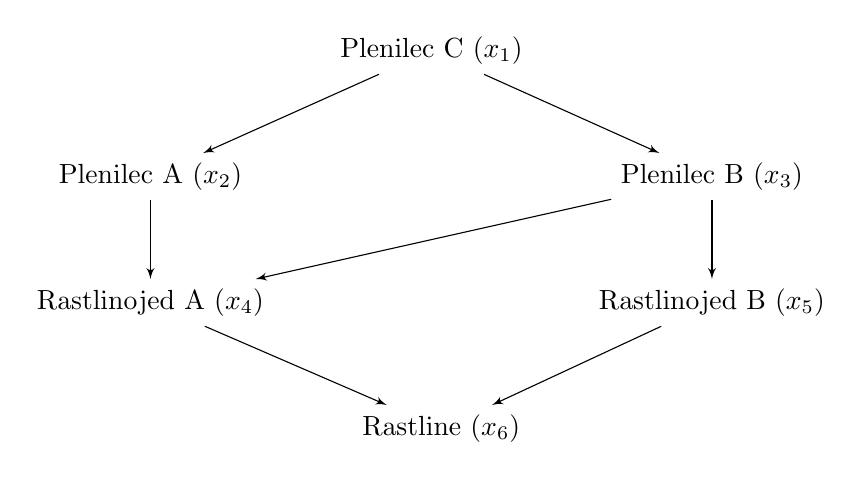
\begin{tikzpicture}
		\tikzset{edge/.style = {->,> = latex'}}
		\node (A) {Plenilec C ($ x_{1} $)};
		\node[below left=of A] (B) {Plenilec A ($ x_{2} $)};
		\node[below right=of A] (C) {Plenilec B ($ x_{3} $)};
		\node[below=of B] (D) {Rastlinojed A ($ x_{4} $)};
		\node[below=of C] (E) {Rastlinojed B ($ x_{5} $)};
		\node[below right=of D] (F) {Rastline ($ x_{6} $)};
		\draw[edge] (A) edge (B) edge (C);
		\draw[edge] (B) edge (D);
		\draw[edge] (C) edge (D) edge (E);
		\draw[edge] (D) edge (F);
		\draw[edge] (E) edge (F);
	\end{tikzpicture}
\end{center}
Puščice označujejo smer prehranjevanja (npr. Plenilec A se prehranjuje z Rastlinojedom A).
Z $ x_{i} $ označimo velikost posamezne populacije. Sprememba velikosti posamezne populacije
je tako odvisna od naravnega prirastka/smrtnosti ($ b_{i} $), smrtnosti zaradi ulova in prirastka zaradi
prehranjevanja z drugo vrsto ($ a_{ij} $). Ulov in prehranjevanje sta odvisna od velikosti ustreznih drugih populacij,
naravni prirastek/smrtnost pa je odvisna samo od velikosti populacije. Dinamiko $ i $-te
populacije lahko opišemo tako:
\begin{equation}
	\dot x_{i} = x_{i}\cdot b_{i} + \sum_{i \not = j} a_{ij}\cdot x_{i}\cdot x_{j}
\end{equation}
kjer je $ x_{i} $ velikost $ i $-te populacije, $ b_{i} $ je koeficient naravnega prirastka/smrtnosti,
$ a_{ij}\cdot x_{i}\cdot x_{j} $ pa je sprememba $ i $-te populacije glede na interakcijo z $ j $-to populacijo.

\section{Reševanje}

\subsection{Naloga 1}
Sistem diferencialnih enačb za naš primer je naslednji:
\begin{align*}
	&\dot x_{1} = x_{1}\cdot(b_{1}+a_{12}\cdot x_{2}+a_{13}\cdot x_{3}) \\
	&\dot x_{2} = x_{2}\cdot(b_{2}+a_{21}\cdot x_{1}+a_{24}\cdot x_{4}) \\
	&\dot x_{3} = x_{3}\cdot(b_{3}+a_{31}\cdot x_{1}+a_{34}\cdot x_{4}+a_{35}\cdot x_{5}) \\
	&\dot x_{4} = x_{4}\cdot(b_{4}+a_{42}\cdot x_{2}+a_{43}\cdot x_{3}+a_{46}\cdot x_{6}) \\
	&\dot x_{5} = x_{5}\cdot(b_{5}+a_{53}\cdot x_{3}+a_{56}\cdot x_{6}) \\
	&\dot x_{6} = x_{6}\cdot(b_{6}+a_{64}\cdot x_{4}+a_{65}\cdot x_{5}) \\
\end{align*}
$ x_{i} $ predstavlja velikost i-te populacije, $ \dot x_{i} $ pa predstavlja spremembo
i-te populacije v nekem trenutku. Velikosti posameznih vrst bomo zapisali v
vektor $ X = \left[x_{1}, x_{2}, x_{3}, x_{4}, x_{5}, x_{6}\right]^{T} $.
Sistem diferencialnih enačb pa bomo zapisali v vektor $ \dot X $:
\begin{equation}
	\dot X =
	\begin{bmatrix}
		\dot x_{1} \\
		\dot x_{2} \\
		\dot x_{3} \\
		\dot x_{4} \\
		\dot x_{5} \\
		\dot x_{6} \\
	\end{bmatrix}
	=
	\begin{bmatrix}
		x_{1}\cdot(b_{1}+a_{12}\cdot x_{2}+a_{13}\cdot x_{3}) \\
		x_{2}\cdot(b_{2}+a_{21}\cdot x_{1}+a_{24}\cdot x_{4}) \\
		x_{3}\cdot(b_{3}+a_{31}\cdot x_{1}+a_{34}\cdot x_{4}+a_{35}\cdot x_{5}) \\
		x_{4}\cdot(b_{4}+a_{42}\cdot x_{2}+a_{43}\cdot x_{3}+a_{46}\cdot x_{6}) \\
		x_{5}\cdot(b_{5}+a_{53}\cdot x_{3}+a_{56}\cdot x_{6}) \\
		x_{6}\cdot(b_{6}+a_{64}\cdot x_{4}+a_{65}\cdot x_{5}) \\
	\end{bmatrix}
\end{equation}
V vektorju $ b = \left[b_{1}, b_{2}, b_{3}, b_{4}, b_{5}, b_{6}\right]^{T} $ so koeficienti naravnega prirastka/smrtnosti,
ki je za rastline ($ x_{6} $) pozitiven, za vse ostale pa negativen. \\
Sistem enačb za dani primer lahko tako zapišemo kot
\begin{equation}
	\dot X = X*(b+A\cdot X)
\end{equation}
($ * $ predstavlja množenje po elementih),
kjer matrika $ A $ vsebuje koeficiente hranjenja in plenjenja $ a_{ij} $:
\begin{equation}
	A =
	\begin{bmatrix}
		0 & a_{12} & a_{13} & 0 & 0 & 0 \\
		a_{21} & 0 & 0 & a_{24} & 0 & 0 \\
		a_{31} & 0 & 0 & a_{34} & a_{35} & 0 \\
		0 & a_{42} & a_{43} & 0 & 0 & a_{46} \\
		0 & 0 & a_{53} & 0 & 0 & a_{56} \\
		0 & 0 & 0 & a_{64} & a_{65} & 0 \\
	\end{bmatrix}
\end{equation}
Koeficient $ a_{ij} $ predstavlja interakcijo vrste $ i $ z vrsto $ j $. Pozitivna vrednost pomeni, da se vrsta
$ i $ prehranjuje z vrsto $ j $, negativna pa, da je vrsta $ i $ plen vrste $ j $. Vrsta s sabo nima take interakcije, zato
so elemeniti, kjer je $ i=j $, enaki $ a_{ij} = 0 $. Koeficienta $ a_{ij} $ in $ a_{ji} $ pa si nista nujno nasprotna, saj lahko plenilska
vrsta poje več plena, kot pa ima koristi od tega. \\
Za začetek smo določili $ b = \left[-0.1, -0.1, -0.1, -0.05, -0.05, 0.3\right]^{T} $
in 
\begin{equation}
	A = 
	\begin{bmatrix}
		0 & 0.5 & 0.7 & 0 & 0 & 0 \\
		-2 & 0 & 0 & 1 & 0 & 0 \\
		-8 & 0 & 0 & 1 & 4 & 0 \\
		0 & -6 & -1 & 0 & 0 & 2 \\
		0 & 0 & -1 & 0 & 0 & 1 \\
		0 & 0 & 0 & -2 & -5 & 0 \\
	\end{bmatrix}\cdot 0.001
\end{equation}

\subsection{Naloga 2}
Stacionarna rešitev sistema je, ko je vektor $ \dot X $ enak  $ 0 $. To pomeni, da je
$ X*(b+A\cdot X) = 0 $. Vektor $ X = 0 $ že zadosti našemu pogoju, vendar iščemo neničelno
rešitev. Za naša $ A $ in $ b $ je to $ X = \left[8.7, 28.7, 122.3, 117.4, 13.0, 172.3\right]^{T} $.
Slika rešitve po 100 iteracijah izgleda tako:\\
\begin{center}
	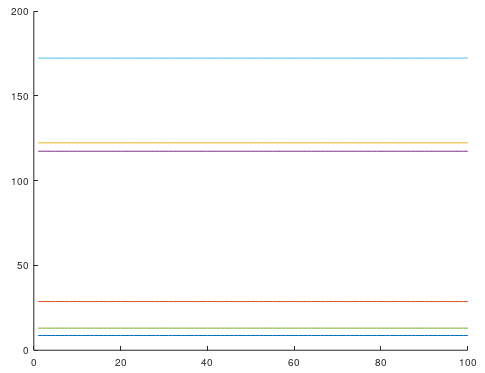
\includegraphics{stationary.png}
\end{center}

\subsection{Naloga 3}
Napisali smo funcijo {\sf simulatePopulation.m}, ki za vhod vzame matriko interakcij $ A $,
vektor naravnih prirastkov $ b $ in začetne velikosti populacij v vektorju $ X $.
\begin{lstlisting}[language=Octave]
function retval = simulatePopulation (x0, b, A, n, fig)
    F = @(X, b, A) X.*(b+A*X); %enacba prirastka za vsako vrsto
    h = 0.1; %dolzina koraka

    tocke = zeros(6, n);
    x = x0;

    %%Simulacija
    for i = (1:n)
        x = x + rk4Step(F, x, h, b, A);
        tocke(:, i) = x;
    end

    figure(fig)
    hold on;
    for i = (1:6)
        vektor = zeros(1, n);
        vektor(1, :) = tocke(i, :);
        plot(vektor);
    endfor

    lastX = x;
endfunction
  
%%Korak rk4
function val = rk4Step(f, x0, h, b, A)
    k1=feval(f, x0, b, A);
    k2=feval(f, x0 + k1*h/2, b, A);
    k3=feval(f, x0 + k2*h/2, b, A);
    k4=feval(f, x0 + k3*h, b, A);
    val = h*(k1+2*k2+2*k3+k4)/6;
endfunction
\end{lstlisting}

\subsection{Naloga 4}
Naredili smo simulacijo za začetne pogoje, ki se malo razlikujejo od $ X $. Dobili smo
$ X_{nov} = \left[9.0, 32.6, 125.9, 121.0, 16.5, 175.4\right]^{T} $, slika simulacije po 5000 iteracijah
pa izleda tako:\\
\begin{center}
	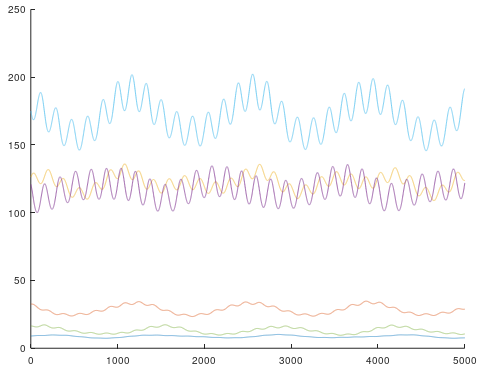
\includegraphics{stationary_almost.png}
\end{center}
Sistem se za naše vrednosti ($ A, b $ in $ X_{nov} $) obnaša ciklično.

\subsection{Naloga 5}
Preučili smo obnašanje sistema za različne vrednosti koeficientov in začetnih pogojev
in našli ciklično obnašanje, asimptotično ciklično obnašanje in kaos.\\
\\
\\
\\
\\
\\
\\
\\
\\
\\
\\
\\
\\
\\
\\
\\
\\
\\
\\
Asimptotično ciklično obnašanje, kjer imamo spiralni lijak, smo dobili z naslednjimi začetnimi vrednostmi:\\
$ A =
\begin{bmatrix}
	0 & 0.37939 & 1.38080 & 0 & 0 & 0 \\
	-1.10424 & 0 & 0 & 0.65246 & 0 & 0 \\
	-0.30582 & 0 & 0 & 1.24509 & 0.40233 & 0 \\
	0 & -0.99713 & -0.73865 & 0 & 0 & 0.39387 \\
	0 & 0 & -0.35715 & -0 & 0 & 0.39208 \\
	0 & 0 & 0 & -1.50798 & -1.78165 & 0 \\
\end{bmatrix} $, \\
$ b =
\begin{bmatrix}
	-3.89109 \\
	-0.27347 \\
	-3.53131 \\
	-6.79120 \\
	-8.91734 \\
	9.72807 \\
\end{bmatrix} $ in
$ X =
\begin{bmatrix}
	0.77988 \\
	1.22798 \\
	2.48059 \\
	1.73900 \\
	3.98827 \\
	25.00319 \\
\end{bmatrix} $. \\
Vektor $ X $ se od stacionarne rešitve sistema razlikuje samo za $ 0.00012384 $. Slika simulacije
sistema s takimi podatki pa je naslednja:
\begin{center}
	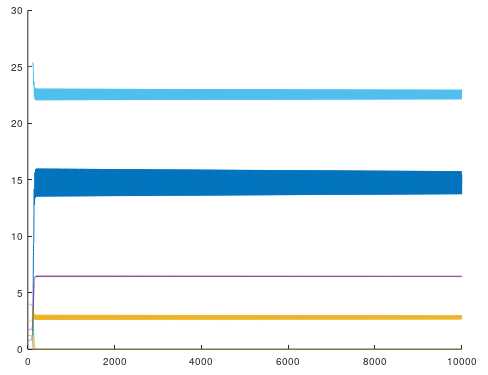
\includegraphics{asimptotic_cyclic_sink.png}
\end{center}
.
\\
\\
\\
\\
\\
\\
\\
\\
Asimptotično ciklično obnašanje s spiralnim izvorom pa smo dobili z naslednjimi
začetnimi vrednostmi:\\
$ A =
\begin{bmatrix}
	0 & 0.000084 & 0.027628 & 0 & 0 & 0 \\
	-0.011626 & 0 & 0 & 0.032503 & 0 & 0 \\
	-0.033349 & 0 & 0 & 0.038057 & 0.028158 & 0 \\
	0 & -0.026921 & -0.033088 & 0 & 0 & 0.028894 \\
	0 & 0 & -0.008998 & 0 & 0 & 0.009693 \\
	0 & 0 & 0 & -0.004489 & -0.006963 & 0 \\
\end{bmatrix} $, \\
$ b =
\begin{bmatrix}
	-0.128572 \\
	-0.023682 \\
	-0.291557 \\
	-0.154676 \\
	-0.198708 \\
	0.164787 \\
\end{bmatrix} $ in
$ X =
\begin{bmatrix}
	14.8432 \\
	15.1853 \\
	4.6090 \\
	6.0374 \\
	19.7722 \\
	24.7789 \\
\end{bmatrix} $. \\
Vektor $ X $ se od stacionarne rešitve razlikuje za $ 0.0023216 $. Slika simulacije
sistema izgleda tako:
\begin{center}
	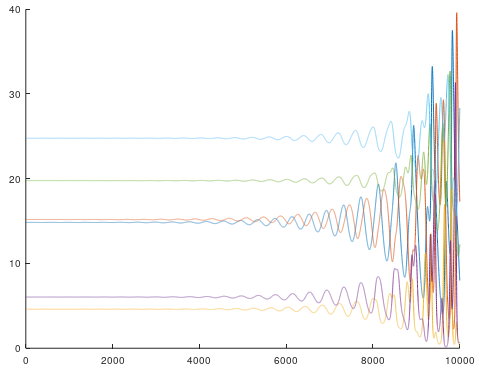
\includegraphics{asimptotic_cyclic_source.png}
\end{center}
.
\\
\\
\\
\\
\\
\\
\\
\\
Kaos smo dobili z naslednjimi koeficienti:\\
$ A =
\begin{bmatrix}
	0 & 0.024710 & 0.024893 & 0 & 0 & 0 \\
	-0.003471 & 0 & 0 & 0.024640 & 0 & 0 \\
	-0.027545 & 0 & 0 & 0.036172 & 0.027497 & 0 \\
	0 & -0.034815 & -0.004165 & 0 & 0 & 0.028781 \\
	0 & 0 & -0.029746 & 0 & 0 & 0.018492 \\
	0 & 0 & 0 & -0.014320 & -0.039922 & 0 \\
\end{bmatrix} $, 
$ b =
\begin{bmatrix}
	-0.245517 \\
	-0.094402 \\
	-0.114666 \\
	-0.113336 \\
	-0.150582 \\
	0.235885 \\
\end{bmatrix} $ in
$ X =
\begin{bmatrix}
	7.2023 \\
	7.9662 \\
	1.7152 \\
	4.6668 \\
	4.4584 \\
	12.1101 \\
\end{bmatrix} $. \\
Vektor $ X $ se od stacionarne rešitve razlikuje za $ 1.9694 $,
za sistem pa po 10000 iteracijah dobimo naslednjo naslednjo sliko:\\
\begin{center}
	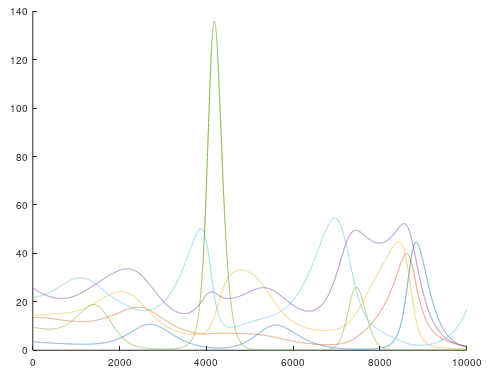
\includegraphics{caos.png}
\end{center}
.
\\
\\
\\
\\
\\
\\
\\
\\
Ciklično obnašanje smo našli z naslednjimi koeficienti:\\
$ A =
\begin{bmatrix}
	0 & 0.021620 & 0.037477 & 0 & 0 & 0 \\
	-0.011555 & 0 & 0 & 0.026287 & 0 & 0 \\
	-0.026978 & 0 & 0 & 0.012645 & 0.027949 & 0 \\
	0 & -0.030686 & -0.019335 & 0 & 0 & 0.041368 \\
	0 & 0 & -0.033011 & 0 & 0 & 0.030491 \\
	0 & 0 & 0 & -0.000749 & -0.012079 & 0 \\
\end{bmatrix} $, 
$ b =
\begin{bmatrix}
	-0.2454399 \\
	-0.2962493 \\
	-0.1088634 \\
	-0.0064447 \\
	-0.1757772 \\
	0.2704713 \\
\end{bmatrix} $ in
$ X =
\begin{bmatrix}
	28.8557 \\
	8.7814 \\
	1.4681 \\
	23.9553 \\
	20.9203 \\
	7.3815 \\
\end{bmatrix} $. \\
Vektor $ X $ se od stacionarne rešitve razlikuje za $ 0.025147 $, slika simulacije pa je naslednja:
\begin{center}
	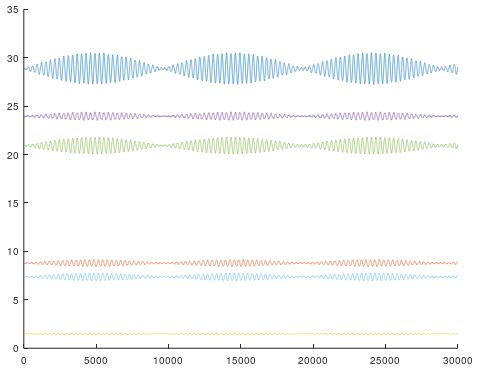
\includegraphics{cycle.png}
\end{center}
.
\\
\\
\\
\\
\\
\\
\\
\\
\\
Obnašanje sistema pa je odvisno od lastnih vrednosti jakobijeve matrike sistema
v stacionarni točki. Jakobijeva matrika je enaka:
\begin{equation}
	J_{x_{1}} =
	\begin{bmatrix}
		b_{1}+x_{2}a_{12}+x_{3}a_{13}+x_{4}a_{14}+x_{5}a_{15}+x_{6}a_{16} \\
		x_{2}a_{21} \\
		x_{3}a_{31} \\
		x_{4}a_{41} \\
		x_{5}a_{51} \\
		x_{6}a_{61} \\
	\end{bmatrix}
\end{equation}
\begin{equation}
	J_{x_{2}} =
	\begin{bmatrix}
		x_{1}a_{12} \\
		b_{2}+x_{1}a_{21}+x_{3}a_{23}+x_{4}a_{24}+x_{5}a_{25}+x_{6}a_{26} \\
		x_{3}a_{32} \\
		x_{4}a_{42} \\
		x_{5}a_{52} \\
		x_{6}a_{62} \\
	\end{bmatrix}
\end{equation}
\begin{equation}
	J_{x_{3}} =
	\begin{bmatrix}
		x_{1}a_{13} \\
		x_{2}a_{23} \\
		b_{3}+x_{1}a_{31}+x_{2}a_{32}+x_{4}a_{34}+x_{5}a_{35}+x_{6}a_{36} \\
		x_{4}a_{43} \\
		x_{5}a_{53} \\
		x_{6}a_{63} \\
	\end{bmatrix}
\end{equation}
\begin{equation}
	J_{x_{4}} =
	\begin{bmatrix}
		x_{1}a_{14} \\
		x_{2}a_{24} \\
		x_{3}a_{34} \\
		b_{4}+x_{1}a_{41}+x_{2}a_{42}+x_{3}a_{43}+x_{5}a_{45}+x_{6}a_{46} \\
		x_{5}a_{54} \\
		x_{6}a_{64} \\
	\end{bmatrix}
\end{equation}
\begin{equation}
	J_{x_{5}} =
	\begin{bmatrix}
		x_{1}a_{15} \\
		x_{2}a_{25} \\
		x_{3}a_{35} \\
		x_{4}a_{45} \\
		b_{5}+x_{1}a_{51}+x_{2}a_{52}+x_{3}a_{53}+x_{4}a_{54}+x_{6}a_{56} \\
		x_{6}a_{65} \\
	\end{bmatrix}
\end{equation}
\begin{equation}
	J_{x_{6}} =
	\begin{bmatrix}
		x_{1}a_{16} \\
		x_{2}a_{26} \\
		x_{3}a_{36} \\
		x_{4}a_{46} \\
		x_{5}a_{56} \\
		b_{6}+x_{1}a_{61}+x_{2}a_{62}+x_{3}a_{63}+x_{4}a_{64}+x_{5}a_{65} \\
	\end{bmatrix}
\end{equation}
\begin{equation}
	JF =
	\begin{bmatrix}
		J_{x_{1}} & J_{x_{2}} & J_{x_{3}} & J_{x_{4}} & J_{x_{5}} & J_{x_{6}} \\
	\end{bmatrix}
\end{equation}
Lastne vrednosti jacobijeve matrike v stacionarni točki so kompleksne. Imaginarni del skrbi za ciklično obnašanje, od njihovega realnega dela pa
je odvisno obnašanje sistema. Če je realni del lastne vrednosti negativen, je stacionarna točka
spiralno privlačna, če je pozitiven, je spiralno odbojna. Če je realni del enak $ 0 $, imamo krožnico.\\
Obnašanje sistema okoli točke, ki ima različno predznačene realne dele lastnih vrednosti, pa je težje opisati. Okoli take točke je več podprostorov,
v katerih se sistem obnaša različno. Vektorski podprostor je stabilen (spiralno privlačen proti točki), če ima lastna vrednost negativen realni del.
Tak prostor razpenjajo ustrezni lastni vektorji. Drug vektorski podprostor je nestabilen (spiralno odbija stran od točke), če ima lastna vrednost poziriven
realni del. Tudi tega razpenjajo pripadajoči lastni vektorji. Vektorski podprostor v okolici stacionarne točke pa je lahko tudi center (sistem kroži), če obstaja
lastna vrednost brez realnega dela. Ta podprostor pa razpenjajo lastni vektorji, ki pripadajo takim lastnim vrednostim.\\
Sistem ima tako splošno rešitev, ki je naslednja:
\begin{equation}
	x(t) = e^{\alpha t}((C_{1}cos(\beta t)+C_{2}sin(\beta t))u+(-C_{1}sin(\beta t)+C_{2}cos(\beta t))w)
\end{equation}
Lastna vrenost Jacobijeve matrike v stacionarni točki takega sistema je oblike $ \lambda_{1,2} = \alpha \pm \beta i $.
V zgornji enačbi je $ \alpha $ realni del lastne vrednosti in $ \beta $ imaginarni del lastne vrednosti.
Vektor $ u $ je realni del lastnega vektorja, $ w $ pa je imaginarni del lastnega vektorja. Ker sta lastni
vrednosti konjugirani, sta konjugirana tudi njuna lastna vektorja, zato v enačbi nastopa samo eden.\\
Ker pa imamo sistem šest spremenljivk, imamo tudi šest lastnih vrednosti ($ \lambda_{1}, \dots, \lambda_{6} $) in šest lastnih vektorjev
($ v_{1}, \dots, v_{6} $). Ker pa so med lastnimi vrednostmi in lastnmi vektorji konjugirani pari, ki jih lahko zapišemo tako:
\begin{align*}
	&\lambda_{1,2} = \alpha_{1} \pm \beta_{1}i \\
	&\lambda_{3,4} = \alpha_{3} \pm \beta_{3}i \\
	&\lambda_{5,6} = \alpha_{5} \pm \beta_{5}i \\
\end{align*}
in
\begin{align*}
	&v_{1,2} = u_{1} \pm w_{1}i \\
	&v_{3,4} = u_{3} \pm w_{3}i \\
	&v_{5,6} = u_{5} \pm w_{5}i \\
\end{align*}
nam da zgornja enačba sistem treh rešitev za naš problem:
\begin{equation}
	x_{1}(t) = e^{\alpha_{1} t}((C_{1}cos(\beta_{1} t)+C_{2}sin(\beta_{1} t))u_{1}+(-C_{1}sin(\beta_{1} t)+C_{2}cos(\beta_{1} t))w_{1})
\end{equation}
\begin{equation}
	x_{3}(t) = e^{\alpha_{3} t}((C_{3}cos(\beta_{3} t)+C_{4}sin(\beta_{3} t))u_{3}+(-C_{3}sin(\beta_{3} t)+C_{4}cos(\beta_{3} t))w_{3})
\end{equation}
\begin{equation}
	x_{5}(t) = e^{\alpha_{5} t}((C_{5}cos(\beta_{5} t)+C_{6}sin(\beta_{5} t))u_{5}+(-C_{5}sin(\beta_{5} t)+C_{6}cos(\beta_{5} t))w_{5})
\end{equation}
splošna rešitev pa je linearna kombinacija le teh:
\begin{equation}
	x(t) = a_{1}x_{1}(t) + a_{3}x_{3}(t) + a_{5}x_{5}(t)
\end{equation}

\end{document}